


%----------------------------------
\chapter{Introduction}\label{ch:NEDintro}
%----------------------------------

\section{Purpose and Objectives of the \NEDDesc}
%%%%%%%%%%%%%%%%%%%%%%%%%%%%%%%%%%%%%%%%%%%%%%%%%%%%%%%%%%%%%%%%%%%%%%%%%%%%%%%%%
%
% Purpose:  Introduction for the NED model.
%
% 
%
%%%%%%%%%%%%%%%%%%%%%%%%%%%%%%%%%%%%%%%%%%%%%%%%%%%%%%%%%%%%%%%%%%%%%%%%%%%%%%%%


%\section{Purpose and Objectives of \NEDDesc}
% Incorporate the intro paragraph that used to begin this Chapter here. 
% This is location of the true introduction where you explain what this model 
% does.

The \NEDDesc\ is used to express the state of a vehicle with respect to some planet (usually the one about which it is orbiting) in terms of planetary North, planetary East, and local Down (with respect to the planet).  The planetary basis can be specified either as spherical (geocentric), or elliptical (geodetic).  For more discussion on the difference between spherical (geocentric) and elliptical (geodetic) representations, see the \textref{Planetary Derived State Model}{ch:planetaryintro}.

While several of the Derived State values simply describe the state of a vehicle in some other defined reference frame, the North-East-Down Derived State also defines the reference frame itself.  The state of the vehicle in the North-East-Down representation is identical to that in the Planetary representation, with both elliptical (geodetic) and spherical (geocentric) representations available.  The North-East-Down reference frame is based on \textit{either} the elliptical \textit{or} the spherical representation; both are not available simultaneously unless two different instances of NedDerivedState are instantiated.

The North-East-Down reference frame, created by this model, is a recti-linear frame, so for two vehicles at the same altitude, the state of one in the NED frame of another will exhibit a ``Down'' component. See Figure~\ref{fig:nedrectilinear} for an illustration.

\begin{figure}[!ht]
\begin{center}
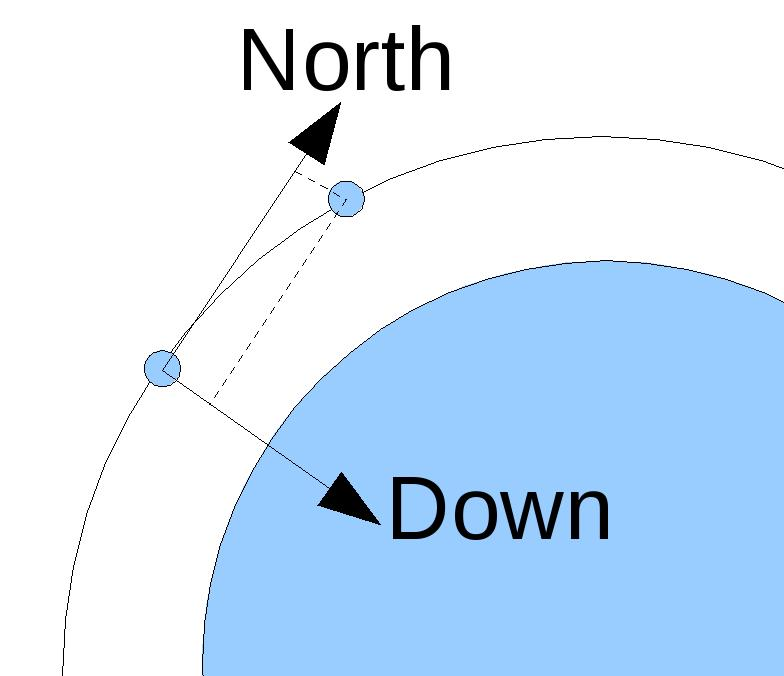
\includegraphics[width=2.5in]{figures/rectilinear.jpg}
\caption{The effect of the curvature of an orbit on the relative state using rectilinear coordinates.}
\label{fig:nedrectilinear}
\end{center}
\end{figure}
















%----------------------------------
\chapter{Product Requirements}\label{ch:NEDreqt}
%----------------------------------


%%%%%%%%%%%%%%%%%%%%%%%%%%%%%%%%%%%%%%%%%%%%%%%%%%%%%%%%%%%%%%%%%%%%%%%%%%%%%%%%%
%
% Purpose:  requirements for the NED model
%
% 
%
%%%%%%%%%%%%%%%%%%%%%%%%%%%%%%%%%%%%%%%%%%%%%%%%%%%%%%%%%%%%%%%%%%%%%%%%%%%%%%%%

% add text here to describe general model requirements
% text is of the form:
\requirement{North-East-Down representation}
\label{reqt:NED}
\begin{description}
  \item[Requirement:]\ \newline
     The North-East-Down Derived State will provide the capability for expressing the state of a vehicle in the North-East-Down oriented reference frame of a planet.
  \item[Rationale:]\ \newline
     Capability from JEOD 1.5.
  \item[Verification:]\ \newline
     Inspection, Test
\end{description}

\requirement{North-East-Down frame generation}
\label{reqt:NED_frame}
\begin{description}
  \item[Requirement:]\ \newline
     The North-East-Down Derived State will provide the capability for generating a reference frame oriented with North, East, and Down, as described in the introduction, through which the state of another vehicle may be expressed.
  \item[Rationale:]\ \newline
     Capability from JEOD 1.5.
  \item[Verification:]\ \newline
     Inspection, Test
\end{description}

\section{Requirements Traceability}

\begin{longtable}[c]{||p{3.5in}|p{3.5in}|}
\caption{Requirements Traceability} \\[6pt]
\hline
{\bf Requirement} & {\bf Inspection and Testing} \\ 
\hline \hline
\endfirsthead
\hline
\endfoot
\caption[]{Requirements Traceability (continued)} \\[6pt]
\hline
{\bf Requirement} & {\bf Inspection and Testing} \\ 
\hline \hline
\endhead
\ref{reqt:NED} - North-East-Down representation &
  Insp.~\ref{test:NED} \\ \hline
\ref{reqt:NED_frame} - North-East-Down frame generation &
  Insp.~\ref{test:NED_frame} \\ \hline

\end{longtable}




%----------------------------------
\chapter{Product Specification}\label{ch:NEDspec}
%----------------------------------

\section{Conceptual Design}
%%%%%%%%%%%%%%%%%%%%%%%%%%%%%%%%%%%%%%%%%%%%%%%%%%%%%%%%%%%%%%%%%%%%%%%%%%%%%%%%%
%
% Purpose:  Conceptual part of Product Spec for the NED model
%
% 
%
%%%%%%%%%%%%%%%%%%%%%%%%%%%%%%%%%%%%%%%%%%%%%%%%%%%%%%%%%%%%%%%%%%%%%%%%%%%%%%%%


%\section{Conceptual Design}
The \NEDDesc\ is used to express the state of a vehicle with respect to a planet-fixed, rotating reference frame in a reference frame oriented with local North, East, and Down directions.  The reference frame is defined by East, parallel to the equator (y-axis); Down, perpendicular to the surface (z-axis); and North (x-axis) completes the right-handed coordinate system.  North is not, in general, aligned with the magnetic field, nor the planetary spin axis.

The calculations associated with representing the state in this way are handled by the North-East-Down subset of the planet-fixed model;  see the \href{file:\JEODHOME/models/utils/planet_fixed/docs/planet_fixed.pdf}{\em Planet-Fixed document}~\cite{dynenv:PLANETFIXED} for details.

%\section{Mathematical Formulations}
%%%%%%%%%%%%%%%%%%%%%%%%%%%%%%%%%%%%%%%%%%%%%%%%%%%%%%%%%%%%%%%%%%%%%%%%%%%%%%%%%
%
% Purpose:  Mathematical Formulation part of Product Spec for the NED model
%
% 
%
%%%%%%%%%%%%%%%%%%%%%%%%%%%%%%%%%%%%%%%%%%%%%%%%%%%%%%%%%%%%%%%%%%%%%%%%%%%%%%%%

\section{Mathematical Formulations}

The \NEDDesc\ contains no independent mathematical formulations; the mathematics utilized by the model is provided by the North-East-Down subset of the planet-fixed model, and by the Reference Frames model;  see the \href{file:\JEODHOME/models/utils/planet_fixed/docs/planet_fixed.pdf}{\em Planet-Fixed} ~\cite{dynenv:PLANETFIXED} and the \href{file:\JEODHOME/models/utils/ref\_frames/docs/ref\_frames.pdf}{\em Reference Frames} ~\cite{dynenv:REFFRAMES} documentation for details.  These documents are also linked as appropriate in the detailed design section of this document.


%\section{Detailed Design}

%%%%%%%%%%%%%%%%%%%%%%%%%%%%%%%%%%%%%%%%%%%%%%%%%%%%%%%%%%%%%%%%%%%%%%%%%%%%%%%%%
%
% Purpose:  Detailed part of Product Spec for the NED model
%
% 
%
%%%%%%%%%%%%%%%%%%%%%%%%%%%%%%%%%%%%%%%%%%%%%%%%%%%%%%%%%%%%%%%%%%%%%%%%%%%%%%%%

\section{Detailed Design}
See the \href{file:refman.pdf}{Reference Manual}\cite{derivedstatebib:ReferenceManual} for a summary of member data and member methods for all classes.  

\subsection{Process Architecture}
The architecture for the \NEDDesc\ is trivial, the \NEDDesc\ methods are largely independent of one another.

\subsection{Functional Design}
This section describes the functional operation of the methods in each class.

The \NEDDesc\ contains only one class:
\begin{itemize}
\classitem{NedDerivedState}
\textref{DerivedState}{ref:DerivedState}

This contains the methods \textit{compute\_ned\_frame}, \textit{set\_use\_alt\_pfix}, \textit{initialize}, and \textit{update}:
\begin{enumerate}

\funcitem{compute\_ned\_frame}
This method utilizes methods from the planet-fixed model, see the \href{file:\JEODHOME/models/utils/planet\_fixed/docs/planet\_fixed.pdf}{\em Planet Fixed} documentation~\cite{dynenv:PLANETFIXED} for details on these methods.

It uses the NorthEastDown methods (from the planet-fixed model) \textit{set\_ned\_trans\_states} and \textit{build\_ned\_orientation} to generate the NED state.  The former, in turn, calls the PlanetFixedPosition method \textit{update\_from\_cart} to convert the Cartesian representation into spherical and elliptical representations.  The latter uses these generated latitude and longitude values to  produce a transformation matrix and corresponding quaternions for going from the planet-fixed reference frame to the NorthEastDown reference frame.

\funcitem{set\_use\_alt\_pfix}
This method sets the flag indicating whether to use the default planet-centered, planet-fixed reference frame associated with the planet or the alternate one, if one is available for the planet.

\funcitem{initialize}
The initialization process comprises the following steps:
\begin{enumerate}
\item{} The generic DerivedState initialization routine is called to establish the naming convention of the reference object (i.e., the planet about which the vehicle is orbiting) and state identifier.
\item{} The DerivedState method \textit{find\_planet} is called (which subsequently calls the  \href{file:\JEODHOME/models/dynamics/dyn_manager/docs/dyn_manager.pdf}{\em Dynamics Manager}~\cite{dynenv:DYNMANAGER}) method of the same name to find a planet by name; that name is stored as \textit{reference\_name}, and is usually assigned in an input file.
\item{} Depending on the value of \textit{use\_alt\_pfix}, the element \textit{pfix\_ptr} is set to either the default planet-fixed reference frame or the alternate planet-fixed reference frame of the planet identified by \textit{reference\_name} and the frame is subscribed.
\item{} The name of the NED state is set as \textit{vehicle\_name.planet\_name.ned}.
\item{} The North-East-Down reference frame is added as a child to the \textit{planet\_centered\_planet\_fixed} frame.
\item{} The North-East-Down frame is registered with the Dynamics manager (optional, user can specify with the \textit{register\_frame} flag, default is true).
\item {} The identified planet is then passed into the initialize method for the PlanetFixedPosition object, \textit{ned\_state} (\textit{ned\_state} is a NorthEastDown state, which inherits from PlanetFixedPosition), which simply records a pointer to the planet just found in the PlanetFixedPosition class (see \href{file:\JEODHOME/models/utils/planet\_fixed/docs/planet\_fixed.pdf}{\em Planet Fixed} documentation~\cite{dynenv:PLANETFIXED}).
\end{enumerate}

\funcitem{update}
This method uses the RefFrame method \textit{compute\_relative\_state} (see \href{file:\JEODHOME/models/utils/ref\_frames/docs/ref\_frames.pdf}{\em Reference Frames} documentation~\cite{dynenv:REFFRAMES}) to calculate the full state of the \textit{subject} in the planet fixed reference frame.  Then, it passes the translational part of that state (i.e. position and velocity) into the \textit{compute\_ned\_frame} method.

\end{enumerate}
\end{itemize}



\chapter{User's Guide}\label{ch:NEDuser}
%----------------------------------
The Analysis section of the User's Guide is intended primarily for
users of pre-existing simulations.  
It contains: 
\begin{itemize}
\item A description of how to modify \NEDDesc\ variables after
the simulation
has compiled, including an in-depth discussion of the input file,
\item An overview of how to interpret (but not edit) the S\_define
file,
\item A sample of some of the typical variables that may be logged.
\end{itemize}


The Integration section of the User's Guide is intended for simulation
developers.
It describes the necessary configuration of the \NEDDesc\
within an
S\_define file, and the creation of standard run directories.  The
latter
component assumes a thorough understanding of the preceding Analysis
section of the user guide.
Where applicable, the user may be directed to selected portions of
Product Specification (Chapter \ref{ch:NEDspec}).

The Extension section of the User's Guide is intended primarily for
developers
needing to extend the capability of the \NEDDesc.  Such users
should have a
thorough understanding of how the model is used in the preceding
Integration section, and of the model
specification (described in Chapter \ref{ch:NEDspec}).


\section{Analysis}
%%%%%%%%%%%%%%%%%%%%%%%%%%%%%%%%%%%%%%%%%%%%%%%%%%%%%%%%%%%%%%%%%%%%%%%%%%%%%%%%%
%
% Purpose:  Analysis part of User's Guide for the NED model
%
% 
%
%%%%%%%%%%%%%%%%%%%%%%%%%%%%%%%%%%%%%%%%%%%%%%%%%%%%%%%%%%%%%%%%%%%%%%%%%%%%%%%%

% \section{Analysis}
\label{sec:neduseranalysis}
It must be reiterated that the \NEDDesc\ does not provide a state for the vehicle with which it is associated, it provides a \textit{reference frame}.  The NedDerivedState does contain a member called \textit{ned\_state}, which contains the state of the reference frame with respect to the parent planet-centered planet-fixed reference frame.  This is identical to the planet-fixed state (PlanetaryDerivedState) of the vehicle with respect to the same planet; it is \textbf{not} the North-East-Down state of the vehicle with respect to the same planet. 

\subsection{Identifying the \NEDDesc}
If the North-East-Down reference frame has been included in the simulation, there will be an instance of \textit{NedDerivedState} located in the S\_define file.  This would typically be found in either the vehicle object (usually if the vehicle is to be described in a North-East-Down sense), or a separate relative-state object (usually if a relative state is to be expressed as such).  There should be an accompanying call to an initialization routine, which takes a reference to the \textit{subject\_body} as one if its inputs, and an accompanying call to an update function.  The essential variables \textit{reference\_name} and \textit{ned\_state.altlatlong\_type} are defined elsewhere, often in the input file.

The North-East-Down reference frame, generated by the \NEDDesc, may also be used to represent the state of another vehicle.  In this case, there will be further inclusion of a RelativeDerivedState instance; see the \textref{RelativeDerivedState User's Guide}{sec:relativeuseranalysis} for details on the implementation of RelativeDerivedState.

Example:
\begin{verbatim}
sim_object{
dynamics/derived_state:    NedDerivedState example_of_ned_state;

(initialization) dynamics/derived_state:
example_of_rel_state_object.example_of_ned_state.initialize (
    Inout DynBody &      subject_body = vehicle_1.dyn_body,
    Inout DynManager &   dyn_manager  = manager_object.dyn_manager);
    
{environment} dynamics/derived_state:
example_of_rel_state_object.example_of_ned_state.update ( )

} example_of_rel_state_object;
\end{verbatim}

Then the input file may have entries comparable to:
\begin{verbatim}
example_of_rel_state_object.example_of_ned_state.reference_name = "Earth";
example_of_rel_state_object.example_of_ned_state.ned_state.altlatlong_type = 
                                                      NorthEastDown::spherical;
\end{verbatim}


\subsection{Editing the \NEDDesc}
The planetary identification, and the planetary surface interpretation (spherical / elliptical) are open to edit by the analyst.

\subsection{Output Data}
The following outputs are available from the \NEDDesc, but once again, these are simply the planetary derived states of the origin of the North-East-Down reference frame.  The strength of the \NEDDesc\ comes in its applicability to a RelativeDerivedState; see the \textref{RelativeDerivedState User's Guide}{sec:relativeuseranalysis} for details on the implementation of RelativeDerivedState.
\begin{verbatim}
example_of_rel_state_object.example_of_ned_state.ned_state.cart_coords[0-2]
example_of_rel_state_object.example_of_ned_state.ned_state.sphere_coords.altitude
example_of_rel_state_object.example_of_ned_state.ned_state.sphere_coords.latitude
example_of_rel_state_object.example_of_ned_state.ned_state.sphere_coords.longitude
example_of_rel_state_object.example_of_ned_state.ned_state.ellip_coords.altitude
example_of_rel_state_object.example_of_ned_state.ned_state.ellip_coords.latitude
example_of_rel_state_object.example_of_ned_state.ned_state.ellip_coords.longitude
\end{verbatim}



%\section{Integration}
%%%%%%%%%%%%%%%%%%%%%%%%%%%%%%%%%%%%%%%%%%%%%%%%%%%%%%%%%%%%%%%%%%%%%%%%%%%%%%%%%
%
% Purpose:  Integration part of User's Guide for the NED model
%
% 
%
%%%%%%%%%%%%%%%%%%%%%%%%%%%%%%%%%%%%%%%%%%%%%%%%%%%%%%%%%%%%%%%%%%%%%%%%%%%%%%%%

 \section{Integration}

Simply including the \NEDDesc\ is straightforward; using it to its full capacity is more challenging.

\subsection{Generating the S\_define}

It should be reiterated that if the desire is simply to express the state of a vehicle with respect to the planet, the NedDerivedState and PlanetaryDerivedState perform the same task.  However, the PlanetaryDerivedState is preferred in this situation, because it does not perform the additional task of generating a reference frame.

The North-East-Down model should be used when the state of a vehicle is desired with respect to some point that is not at the center of the planet, e.g., a launch facility.  Under these circumstances, it becomes necessary to instantiate both a NedDerivedState, and a RelativeDerivedState, with the understanding that the NedDerivedState must be evaluated before the RelativeDerivedState (otherwise the RelativeDerivedState output will be based on an out-of-date orientation of the NED reference frame).

An important consequence of using a RelativeDerivedState to express the relative states of two objects in a North-East-Down reference frame requires the consideration of the class structure of both NedDerivedState and RelativeDerivedState.  There are two types of reference frames in use, BodyRefFrame, and RefFrame.  The BodyRefFrame is associated with a DynBody (a body with dynamic properties), while the RefFrame need not be, it can be associated with some fixed (non-dynamic) body or point.

The North-East-Down reference frame in a NedDerivedState is an instance of a RefFrame, there is no requirement that this be attached to a DynBody.  However, the RelativeDerivedState contains both a BodyRefFrame (\textit{subject\_frame}) and a RefFrame (\textit{target\_frame}); the intention is that the state of a body can be expressed in some other reference frame. Therefore, when generating the relative states, it is \textit{not} possible to use the generated North-East-Down reference frame as the subject frame, it must instead be the target frame.  Then, the vehicle whose state is being expressed must be associated with the subject frame, and the \textit{subject\_frame\_name} and \textit{target\_frame\_name} must be set appropriately.  Then, the \textit{direction\_sense} of the Relative Derived State must be \textit{ComputeSubjectStateinTarget}.

An illustration of this is found in the verification simulations for the North-East-Down model (verif/SIM\_NED).  Here, the relative state instance that expresses the state of vehicle1 (\textit{veh}) with respect to vehicle2 (\textit{veh2}), \textit{veh\_wrt\_veh2}, has:
\begin{verbatim}
subject_frame_name = "vehicle1.composite_body";
target_frame_name = "vehicle2.Earth.ned";
direction_sense = RelativeDerivedState::ComputeSubjectStateinTarget;
\end{verbatim}

Notice also in these simulations that the NedDerivedState is contained within the respective vehicle object, while the RelativeDerivedState is contained within the \textit{rel\_state} object.  This assignment is intentional, though not necessary.  What is necessary is that the state of the two vehicles be evaluated before the relative state, and that the NED reference frame be appropriately oriented, based on the state of its parent vehicle, before the relative state can be expressed in that frame.  Therefore, it was chosen to move the relative state calculations to the end of the S\_define, where they will be processed only after the vehicle and NED reference frames have been processed.  This is recommended procedure.

\subsection{Generating the Input File}
The input file (or Modified Data file) must contain the name of the planet, identified as \textit{reference\_name}, and the identification of whether the North-East-Down reference frame should be based on a spherical (geocentric) or elliptical (geodetic) surface.
\begin{verbatim}
example_of_rel_state_object.example_of_ned_state.reference_name = "Earth";
example_of_rel_state_object.example_of_ned_state.ned_state.altlatlong_type = 
                                                       NorthEastDown::spherical;
\end{verbatim}
or
\begin{verbatim}
example_of_rel_state_object.example_of_ned_state.reference_name = "Earth";
example_of_rel_state_object.example_of_ned_state.ned_state.altlatlong_type = 
                                                     NorthEastDown::elliptical;
\end{verbatim}

The user may specify which planet-centered, planet-fixed reference frame (default or alternate) to use as the basis of the relative state calculations for the North-East-Down reference frame. Note: this only works with Planets that have an alternate reference frame defined.
\begin{verbatim}
example_of_rel_state_object.example_of_ned_state.set_use_alt_pfix(False);

\end{verbatim}
or
\begin{verbatim}
example_of_rel_state_object.example_of_ned_state.set_use_alt_pfix(True);

\end{verbatim}

\subsection{Logging the Data}
See the \textref{Analysis}{sec:neduseranalysis} section for a list of available output data, although again, typically, the desired output results from the relative state implementation of the NED reference frame, rather than from the NED state.  See the \textref{Analysis}{sec:relativeuseranalysis} section for a list of available output data from a RelativeDerivedState.


%\section{Extension}
%%%%%%%%%%%%%%%%%%%%%%%%%%%%%%%%%%%%%%%%%%%%%%%%%%%%%%%%%%%%%%%%%%%%%%%%%%%%%%%%%
%
% Purpose:  Extension part of User's Guide for the NED model
%
% 
%
%%%%%%%%%%%%%%%%%%%%%%%%%%%%%%%%%%%%%%%%%%%%%%%%%%%%%%%%%%%%%%%%%%%%%%%%%%%%%%%%

 \section{Extension}

The \NEDDesc\ is not intended to be extensible.  A potential area for further development may be the addition of a comparable reference frame, such as East-North-Up, but this would be a separate entity, not an extension of the NED reference frame.

%----------------------------------
\chapter{Verification and
Validation}\label{ch:NEDivv}
%----------------------------------

\section{Verification}
%%%%%%%%%%%%%%%%%%%%%%%%%%%%%%%%%%%%%%%%%%%%%%%%%%%%%%%%%%%%%%%%%%%%%%%%%%%%%%%%%
%
% Purpose:  Verification part of V&V for the NED model
%
% 
%
%%%%%%%%%%%%%%%%%%%%%%%%%%%%%%%%%%%%%%%%%%%%%%%%%%%%%%%%%%%%%%%%%%%%%%%%%%%%%%%%

% \section{Verification}

%%% code imported from old template structure
\subsection{Inspection of Modeling Requirements}


\inspection{State Encapsulation}\label{inspect:NED}
 The \NEDDesc\ is capable of outputting data as desired, as demonstrated in simulations located at \textit{derived\_state/verif/SIM\_NED/}, thereby satisfying
 requirement \ref{reqt:NED} at the inspection level.

\inspection{Frame Generation}\label{inspect:NED_frame}
 The \NEDDesc\ is capable of generating a reference frame, as demonstrated in simulations located at \textit{derived\_state/verif/SIM\_NED/}, thereby satisfying
 requirement \ref{reqt:NED_frame} at the inspection level.


\subsection{Verification of Model}

 For testing the \NEDDesc, a simulation of two vehicles was established in which the two vehicles are separated by 1 degree on a common orbital trajectory. Both vehicles generate a North-East-Down reference frame, and the relative state of the other vehicle is calculated for both.

\test{Verification of \NEDDesc\ Output Data for Generic Orbits}\label{test:NED}

\begin{description}
\item{Purpose:}\newline
To demonstrate that the data output by the \NEDDesc\ provides meaningful data.

\item{Requirements:}\newline
Satisfactory conclusion of this test satisfies requirement \ref{reqt:NED}

\item{Procedure:}\newline
The data from the North-East-Down output was compared against that from a Planetary Derived State for an identical orbit.  Polar, inclined, and equatorial orbital characteristics were each tested.

\item{Predictions:}
The state output from this simulation should match that from a Planetary Derived State, which has been verified independently in the \textref{PlanetaryDerivedState Verification Section}{ch:planetaryvv}.

\item{Results:}
There appeared to be no, or negligible, differences between the two states. 
\end{description}



\test{Verification of the reference frame orientation}\label{test:NED_frame}
\begin{description}
\item{Purpose:}\newline
To demonstrate that the reference frame generated by the \NEDDesc\ is oriented along the intended axes.

\item{Requirements:}\newline
Satisfactory conclusion of this test satisfies requirement \ref{reqt:NED_frame}

\item{Procedure:}\newline
The relative state data between the two vehicles was compared against theoretical prediction for consistency for polar, inclined, and equatorial orbital characteristics.

\item{Predictions:}
\begin{enumerate}
 \item {Polar orbit.}  
  \begin{enumerate}
   \item{North.} The lead vehicle should be North of the trailing vehicle while latitude is increasing, and South of the trailing vehicle while the latitude is decreasing.  The transition should be sharp, though not coincident between the two frames; as the vehicles cross the pole, the state of the trailing vehicle in the NED frame associated with the lead vehicle should transition first, resulting in a short time when both vehicles are north (or south) of each other. 
   \item {East.}  The relative states should show zero East component in their respective positions.
   \item {Down.}  Because the NED states are rectilinear, both vehicles should be represented as having a state with a positive down component at all times.  See Figure~\ref{fig:nedrectilinear} for a partial illustration of this counter-intuitive phenomenon.  The behavior is also dependent upon the planetary geometry:
   \begin{itemize}
    \item {Spherical.}  The Down component should be constant, at a value equal to $r - r \cos \Delta \theta$.  For these simulations, this value equates to $1.03 km$. 
    \item {Elliptical.} The Down component should oscillate.  In these simulations, the orbit is approximately circular, whereas the definition of \textit{down} is elliptical.  As the vehicles leave the equator, the trailing vehicle should be significantly further below the leading vehicle than the leading vehicle below the trailing vehicle.  As the vehicles approach the poles, the two values should equalize to $1.03 km$, due to symmetry, then drift apart again heading back to the equator; this time, however, the leading vehicle should have the larger down component.  As the vehicles approach the equator again, the values should again equalize, again due to symmetry.  An exaggerated illustration of this is shown in Figure~\ref{fig:nedellipticalrectilinear}.

\begin{figure}[!ht]
\begin{center}
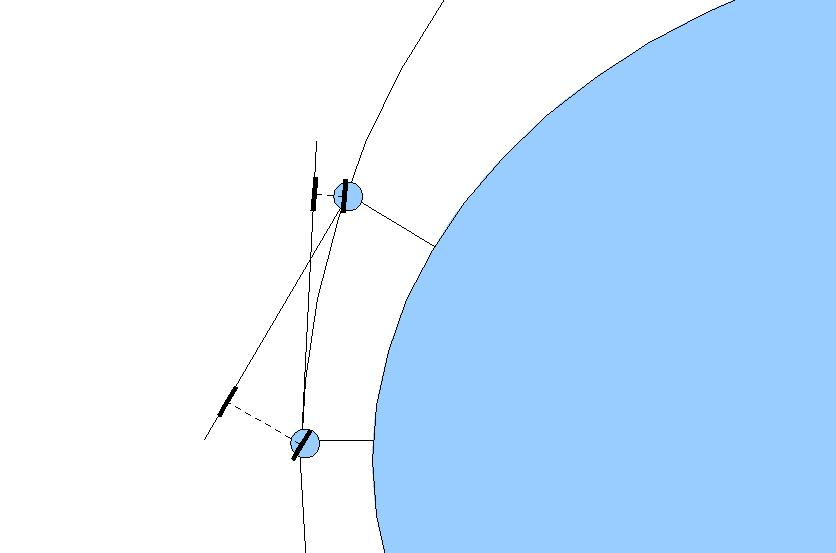
\includegraphics[width=5in]{figures/ned_elliptical_rectilinear.jpg}
\caption{The effect of the difference between the curvature of an orbit and that of the reference ellipse on the relative state using rectilinear coordinates.  The vehicle closer to the equator will exhibit a larger down component in its state than the vehicle farther from the equator.}
\label{fig:nedellipticalrectilinear}
\end{center}
\end{figure}

   \end{itemize}
  \end{enumerate}
 \item {Inclined orbit.}
  \begin{enumerate}
   \item{North.}  As for the polar orbit, the lead vehicle should be North of the trailing vehicle while latitude is increasing, and South of the trailing vehicle while the latitude is decreasing.  Conversely, the transitions at the poles will differ from those observed for the polar orbit; for the inclined orbit, the North component of the relative state should be oscillatory, and ninety degrees out-of-phase from the latitude measurement (so that the North component of the relative state reaches an extremum when the vehicles are at the equator, and goes to zero when the vehicles are at their extreme latitudes).  
   \item {East.}  The lead vehicle should always be East of the trailing vehicle, and the trailing vehicle negative-East of the lead vehicle.
   \item {Down.} By the same argument put forth for the polar orbit, both vehicles should be represented as having a state with a positive down component at all times, constant for spherical geometry and oscillating (though with smaller magnitude due to the variation of the curvature being less significant on an inclined orbit) for the elliptical geometry.  
  \end{enumerate}


 \item {Equatorial orbit.}  
  \begin{enumerate}
   \item{North.} Both relative states should have zero North component.
   \item {East.} The lead vehicle should always be East of the trailing vehicle, and the trailing vehicle negative-East of the lead vehicle.
   \item {Down.} By the same argument put forth for the polar orbit, both vehicles should be represented as having a state with a positive down component at all times, but now be constant for both spherical and elliptical geometries.  
  \end{enumerate}




\end{enumerate}


\item{Results:}
\begin{enumerate}
 \item {Polar orbit.} \ \newline
   The results were mostly as expected.  Figures~\ref{fig:nedpolarell} and \ref{fig:nedpolarellzoom} show the results from the elliptical-geometry reference frame, and Figure~\ref{fig:nedpolarsph} the results from the spherical-geometry reference frame.
  \begin{enumerate}
   \item{North.} The instantaneous switch is seen at polar crossings, with the offset between the two states illustrated better in Figure~\ref{fig:nedpolarellzoom}.  This is at a South pole crossing, and it is clear that the trailing vehicle first transitions to being South of the leading vehicle, then the leading vehicle transitions to being North of the trailing vehicle.
   \item {East.}  The East component is not uniformly zero, it has some instantaneous spikes in its value.  This is attributed to numerical error; those spikes all occur as the vehicles transit the poles, where North and East are not well defined.  
   \item {Down.} For the spherical geometry, the down component shows some oscillation, but that oscillation has magnitude less than $1 cm$, and the mean has the expected value of $1.03 km$.  For the elliptical geometry, the oscillation can clearly be seen.  Figure~\ref{fig:nedpolarellzoom} shows the oscillation from equator heading North (trailing vehicle has larger down component), through the pole at about $1400 s$, then back South to the equator again at approximately $2800 s$.
  \end{enumerate}

\begin{figure}[!ht]
\begin{center}
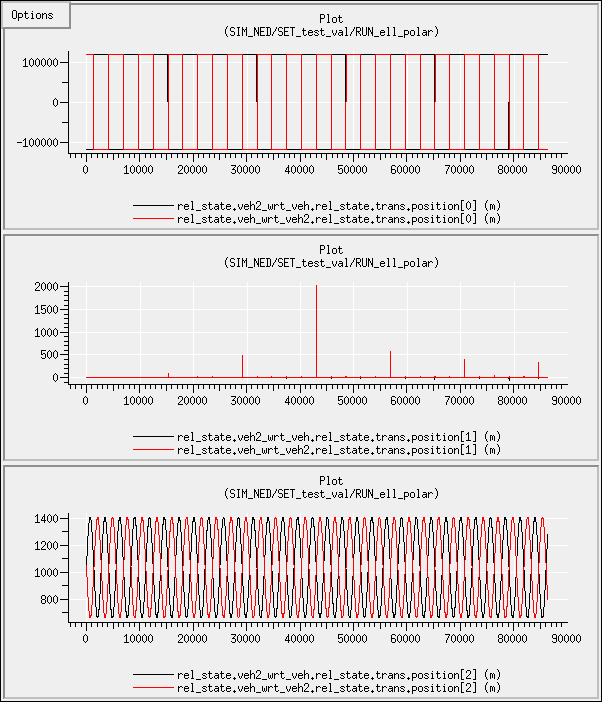
\includegraphics[width=5in]{figures/ned_polar_ell.jpg}
\caption{The relative states for a polar orbit, with elliptical geometry used to define the reference frame.}
\label{fig:nedpolarell}
\end{center}
\end{figure}

\begin{figure}[!ht]
\begin{center}
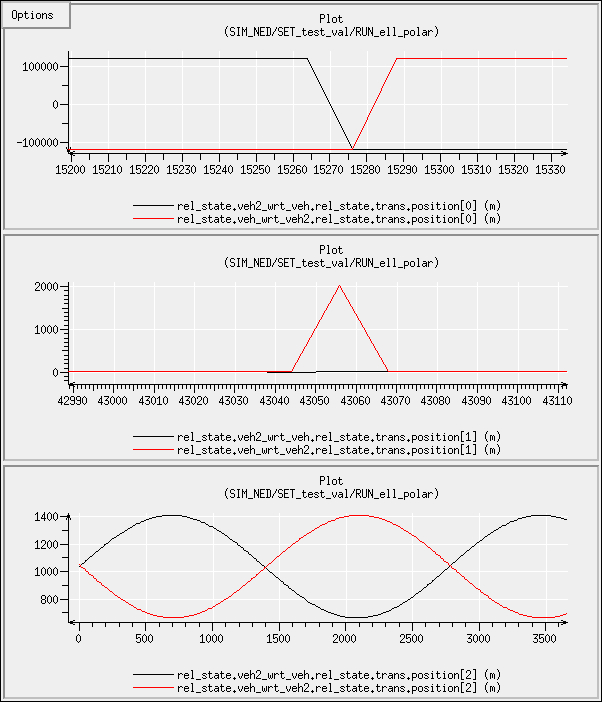
\includegraphics[width=5in]{figures/ned_polar_ell_zoom.jpg}
\caption{The relative states for a polar orbit, with elliptical geometry used to define the reference frame, zoomed in to locations of interest.}
\label{fig:nedpolarellzoom}
\end{center}
\end{figure}

\begin{figure}[!ht]
\begin{center}
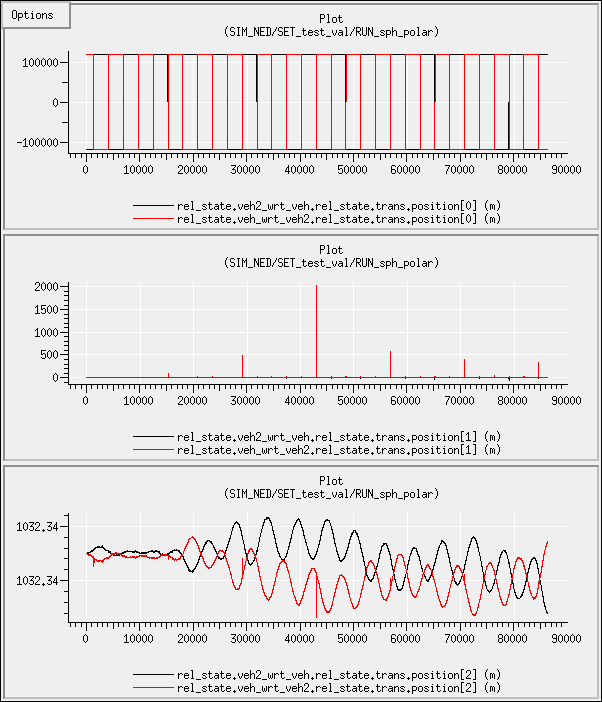
\includegraphics[width=5in]{figures/ned_polar_sph.jpg}
\caption{The relative states for a polar orbit, with spherical geometry used to define the reference frame.}
\label{fig:nedpolarsph}
\end{center}
\end{figure}

\clearpage

\item {Inclined Orbit.} \ \newline
  The results match with expectation.  Figure~\ref{fig:nedincsph} shows the North and East components with the latitude history.  The Down components had a similar oscillation to those seen in the polar orbit and are not shown. A small difference exists of order meters between the North components of the spherical and elliptical geometries, East shows no dependence on geometry, and Down shows a large dependence, as it did in the polar orbit.


\begin{figure}[!ht]
\begin{center}
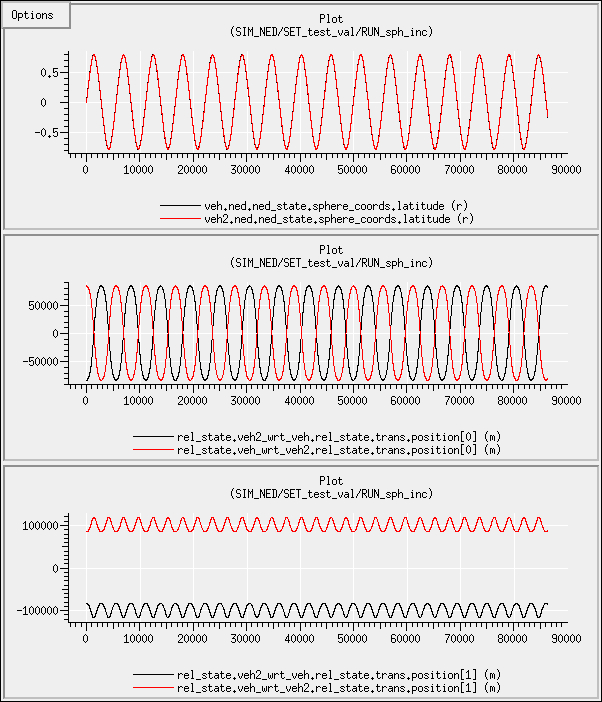
\includegraphics[width=5in]{figures/ned_inc_sph.jpg}
\caption{The variation with time of latitude and of the North and East components of the relative states for an orbit inclined at 45 degrees, with spherical geometry used to define the reference frame.}
\label{fig:nedincsph}
\end{center}
\end{figure}

\clearpage

\item{Equatorial Orbit.}\ \newline
  The results match with expectation.  Figure~\ref{fig:nedequsph} shows the state components; there was no noticeable difference between the spherical and elliptical geometries.
\end{enumerate}

\begin{figure}[!ht]
\begin{center}
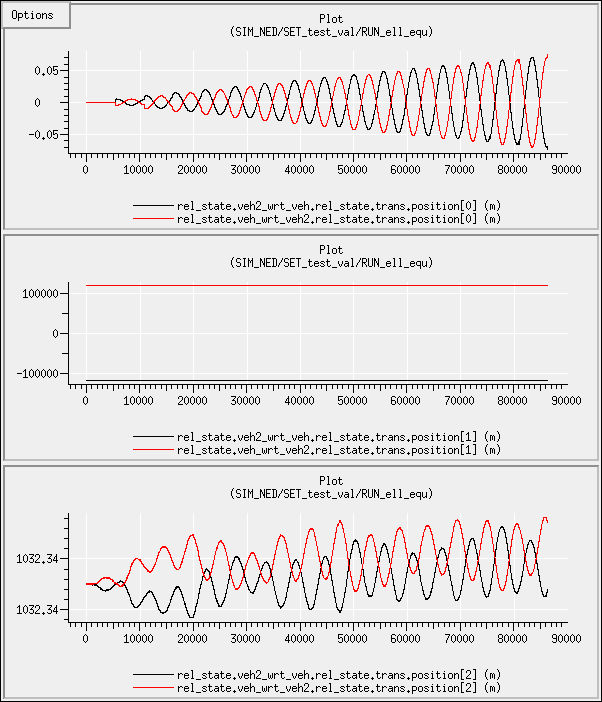
\includegraphics[width=5in]{figures/ned_equ_sph.jpg}
\caption{The relative states for an equatorial orbit with spherical geometry used to define the reference frame.}
\label{fig:nedequsph}
\end{center}
\end{figure}

\end{description}





%\section{Validation}
%%%%%%%%%%%%%%%%%%%%%%%%%%%%%%%%%%%%%%%%%%%%%%%%%%%%%%%%%%%%%%%%%%%%%%%%%%%%%%%%%
%
% Purpose:  Validation part of V&V for the NED model
%
% 
%
%%%%%%%%%%%%%%%%%%%%%%%%%%%%%%%%%%%%%%%%%%%%%%%%%%%%%%%%%%%%%%%%%%%%%%%%%%%%%%%%

\section{Validation}

There is no independent validation of this model.
%%% code imported from old template structure
%\test{<Title>}\label{test:<label>}
%\begin{description}
%\item[Purpose:] \ \newline
%<description>
%\item[Requirements:] \ \newline
%By passing this test, the universal time module 
%partially satisfies requirement~\ref{reqt:<label1>} and 
%completely satisfies requirement~\ref{reqt:<label2>}.
%\item[Procedure:]\ \newline
%<procedure>
%\item[Results:]\ \newline
%<results>
%\end{description}




